% -------------------------------------------------------------------------------- %

\begin{exercise}[Boxplot and quantiles]

Two novel randomized algorithms ($A$ and $B$) are to be compared regarding their runtimes.
Both algorithms were executed $n$ times.
The runtimes (in seconds) are stored in the file \texttt{algorithms.Rdata}

\begin{enumerate}[label = (\alph*)]

    \item Set the working directory and load the data using \texttt{load()}.
    Create a boxplot to compare the running times.
    Color the boxes and add proper notations (axes notations, title etc.).
    More info via \texttt{?boxplot}

    \item Comment on the following statements / questions only using the graphic
    
    \begin{enumerate}[label = (\alph*)]
        \item The first quartile of the times in $A$ was about?
        \item the interquartile range of the times in $B$ is about trice the interquartile range of $A$
        \item Is $n = 100$?
        \item More than half of the running times in $B$ were faster than $3/4$ of the running times in $A$.
        \item At least $50 \%$ in $A$ were faster than the $25 \%$ slowest in $B$.
        \item At least $60 \%$ in $A$ were faster than the $25 \%$ slowest in $B$.
    \end{enumerate}

    \item Regarding the runtimes
    
    \begin{align*}
        23.7, 13.7, 7.6, 9.0, 44.3, 3.5, 2.2, 34.2
    \end{align*}

    which are a subset of $B$, find all empirical
    \begin{enumerate*}
        \item medians,
        \item first quartiles and
        \item $2/3$-qua\underline{n}tiles
    \end{enumerate*}
    (not using \texttt R).

\end{enumerate}

\end{exercise}

% -------------------------------------------------------------------------------- %

\begin{solution}

\phantom{}

\begin{enumerate}[label = (\alph*)]

    \item \phantom{}

    \begin{center}
        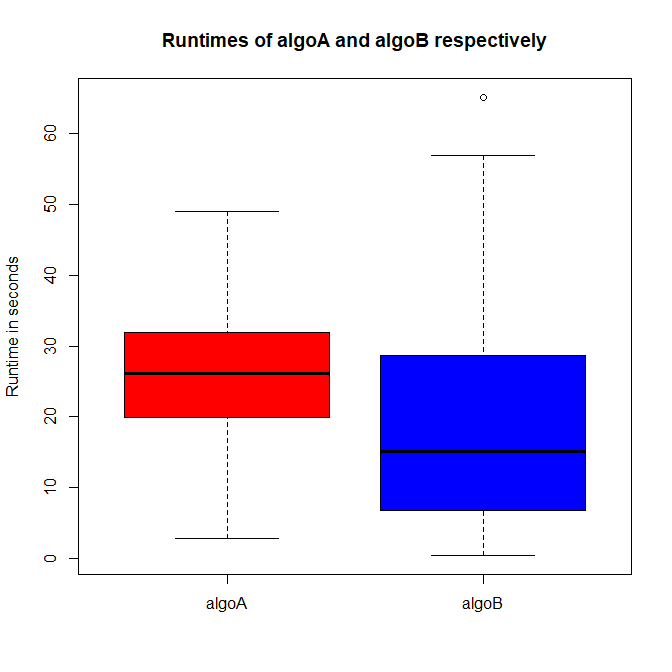
\includegraphics[width = 0.75 \textwidth]{10.5.png}        
    \end{center}

    \lstinputlisting[firstline = 3, lastline = 8]{10.5.r}

    \item

    \begin{enumerate}[label = (\alph*)]

        \item The first quartile of the times in $A$ is $\approx 20$.

        \item I would say twice, but not thrice!

        \item Unclear.
        One cannot tell by looking at the graphic alone.

        \item Yes.
        Consider the blue box, what is below and a little bit what is above.
        Compare this to the red box, and what is above.

        \item Yes.
        Consider the lower half of the red box and what is below.
        Compare this to what is above the blue box.

        \item Unclear.
        The previous argument cannot be applied for certain.

    \end{enumerate}

    \item First of, we will sort the runtimes ascendingly:
    
    \begin{align*}
        1.1, 3.5, 7.6, 9.0, 13.7, 23.7, 34.2, 44.3;
    \end{align*} 

    From this list, we can easily identify the empirical
    
    \begin{enumerate}
        \item medians: $9.0$ and $13.7$,
        \item first quartiles: $3.5$ and $7.6$, and
        \item $2/3$-quantile: $23.7$.
    \end{enumerate}

\end{enumerate}

\end{solution}

% -------------------------------------------------------------------------------- %
